\chapter{Results and performance}
\label{Chapter5}
\lhead{Chapter 5. \emph{Results and performance}}

%\todo{Present the results and discuss any differences between the findings and your initial predictions/hypothesis}

%\todo{Interpret your experimental results - do not just present lots of data and expect the reader to understand it.
%Evaluate what you have achieved against the aims and objectives you outlined in the introduction}

\section{Hypothesis}
As mentionned in Section \ref{section:research_obj}, the primary objective was to implement a new algorithm to find solutions without imposing time constraints. Only instances ($I_1, \ldots, I_8$) are studied because they represent realistic scenarios.

Hence, simulations for every instances have been conducted, testing different combinations of parameters in what is called a grid search. Each combination of parameters was run 10 times to ensure the reliability and consistency of the results.
One challenge, is that the computational budget is limited when using Python. Especially for the more complex instances, ($I_7 \ldots I_{14}$) where the time to find a solution for a given set of parameters is more than 20 minutes. It becomes practically impossible to perform for each instance, 10 simulations for every combination of parameters in the grid search. Hence, the size of the grid search for the more complex instances were reduced as shown in Table \ref{table:Grid search}.

\begin{table}[!ht]
    \centering
    \caption{Grid search}
    \resizebox{\textwidth}{!}{ % Resize the table to fit the text width
        \begin{tabular}{||>{\centering\arraybackslash}p{3cm}
            >{\centering\arraybackslash}p{4.5cm}
            >{\centering\arraybackslash}p{3.5cm}
            >{\centering\arraybackslash}p{2cm}||}
            \toprule
                                        & ($I_1 \ldots I_6$)        & ($I_7 \ldots I_8$) & ($I_9 \ldots I_{14}$) \\ [1ex]
            \midrule
            \textit{selection\_policy}  & top\_k, ratio\_k          & top\_k, ratio\_k   & -                     \\
            \textit{simulation\_policy} & random, greedy, tolerance & greedy             & -                     \\
            \textit{selection\_policy}  & UCB, UCB1T                & UCB, UCB1T         & -                     \\
            \textit{C\_p}               & 0, 1.4, 2.8               & 1.4                & -                     \\
            \textit{N\_children}        & 5, 10, 15                 & 10                 & -                     \\
            \textit{Ratio c}            & 0, .3, .5, .8, 1          & .5                 & -                     \\
            \bottomrule
        \end{tabular}
    }
    \label{table:Grid search}
\end{table}

\section{Results analysis}
\subsection{Overview}

After running the various simulations with the grid search parameters defined in Table \ref{table:Grid search}, our results were compared with those of Kiwi and RL (Reinforcement Learning) \cite{reinforcement_learning_yaro} - the only two official publications about this challenge.

\begin{table}[!ht]
    \centering
    \caption{Best results vs State of the art}
    \resizebox{.8\textwidth}{!}{ % Resize the table to fit the text width
        \begin{tabular}{||>{\centering\arraybackslash}p{1.5cm}
            >{\centering\arraybackslash}p{1.5cm}
            >{\centering\arraybackslash}p{1.5cm}
            >{\centering\arraybackslash}p{1.5cm}
            >{\centering\arraybackslash}p{1.5cm}
            >{\centering\arraybackslash}p{1.5cm} ||}
            \toprule
            Instance & Best known & Best found    & Gap (\%) & Mean & Std   \\ [1ex]
            \midrule
            $I_1$    & 1396       & \textbf{1396} & 0        & 0    & 0     \\
            $I_2$    & 1498       & \textbf{1498} & 0        &      &       \\
            $I_3$    & 7672       & \textbf{7672} & 0        &      &       \\
            $I_4$    & 13952      & 15101         & 8.24     &      & 520.8 \\
            $I_5$    & 690        & -             & -        &      & -     \\
            $I_6$    & 2159       & -             & -        &      & -     \\
            $I_7$    & 30937      & -             &          &      &       \\
            $I_8$    & 4052       & \textbf{4037} & -0.52    &      &       \\
            \bottomrule
        \end{tabular}
    }
    \label{table:Best result vs state of the art}
\end{table}

A solution was found for $I_1, I_2, I_3, I_4,I_7$ and $I_8$. The results shown in table \ref{table:Best result vs state of the art} are the best found costs' solution within the grid search. The results of the simulations for $I_1, I_2, I_3$ are displayed in Section \ref{AppendixC} and the detailed path-solution for $I_1,\ldots, I_8$ (except $I_5, I_6$) can be found in Section \ref{AppendixD}.
\newpage
\subsection{Analysis}
\subsubsection{$I_1$, $I_2$, $I_3$ and $I_4$}
For these instances, solutions were found and the various simulations were carried out successfully. Therefore, the influence of the parameters on the $\mathcal{MCTS}$ function and final solution was investigated. For $I_3$, the analysis focuses on the $C_p$ parameter, the influence of the expansion ratio and finally, the study will investigate the overall correlation matrix.

\subsubsection*{Analysis on $C_p$}
\begin{figure}[!ht]
    \centering
    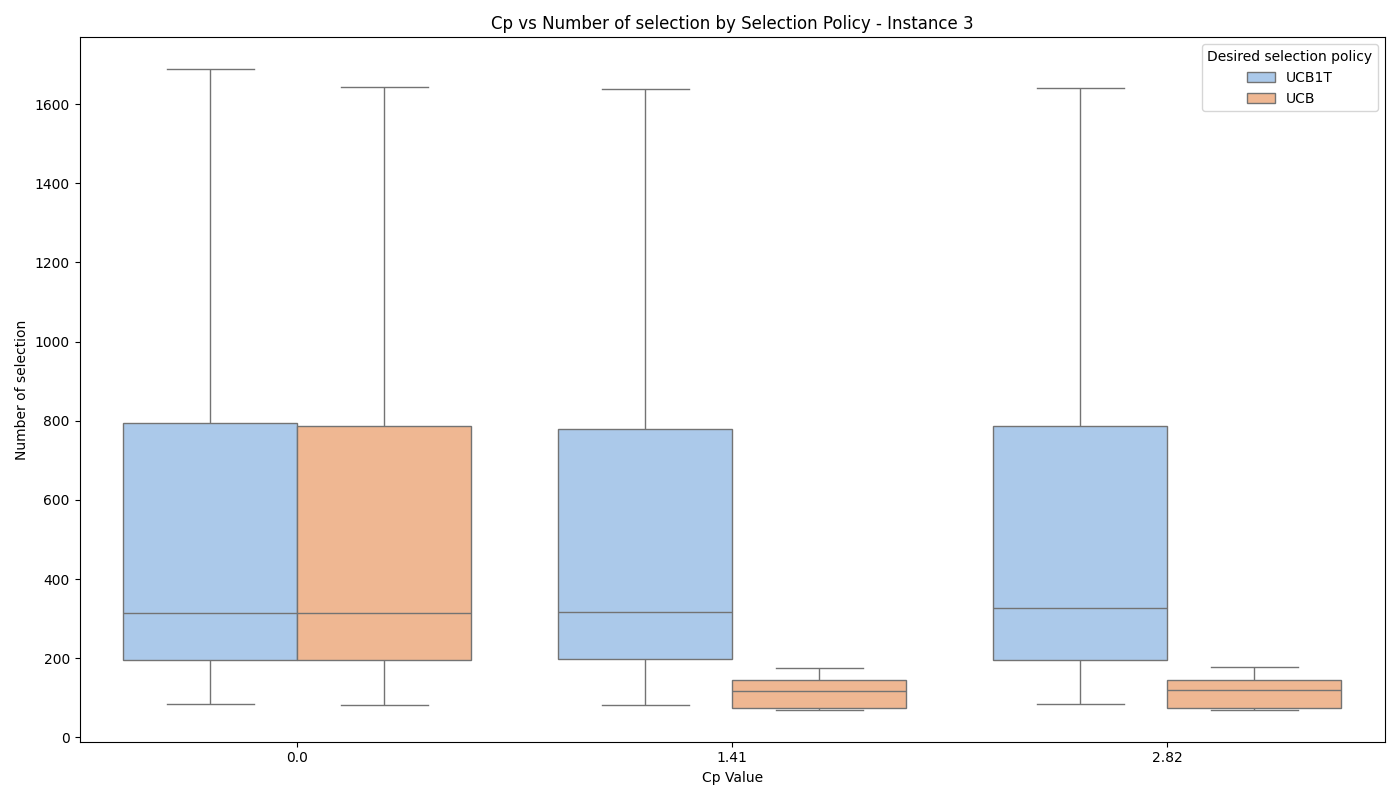
\includegraphics[width=\textwidth]{Figures/3 - cp_vs_selection.png}
    \caption{$C_p$ vs Number of selection}
    \label{fig:cp_vs_selection_3}
\end{figure}

In Figure \ref{fig:cp_vs_cost_3}, the box plots illustrate the relationship between the exploration constant \( C_p \) and the number of selection phases under the UCB and UCB1T selection policies:

\begin{itemize}
    \item \textbf{\( C_p = 0 \) lead to the same performance:}
          When the $C_p=0$, the selection policy of the UCB and the UCB1T are equal (cf equation \ref{eq:UCB} and \ref{eq:UCB1T}).
    \item \textbf{Higher \( C_p \) values lead to faster convergence for UCB:}
          As \( C_p \) increases from $0.0$ to $2.82$, the median number of selection phases under the UCB policy decreases.

    \item \textbf{UCB1T encourages more exploration:}
          UCB1T consistently results in a higher number of selection phases compared to UCB, especially at higher \( C_p \) values. This is consistent with UCB1T's definition to promote broader exploration before converging.
\end{itemize}

Although a higher exploration parameter $C_p$ may lead to faster convergence under the UCB selection policy, it often results in worse outcomes compared to the UCB1T algorithm, as shown in Figure \ref{fig:cp_vs_cost_3}.
\begin{figure}[!ht]
    \centering
    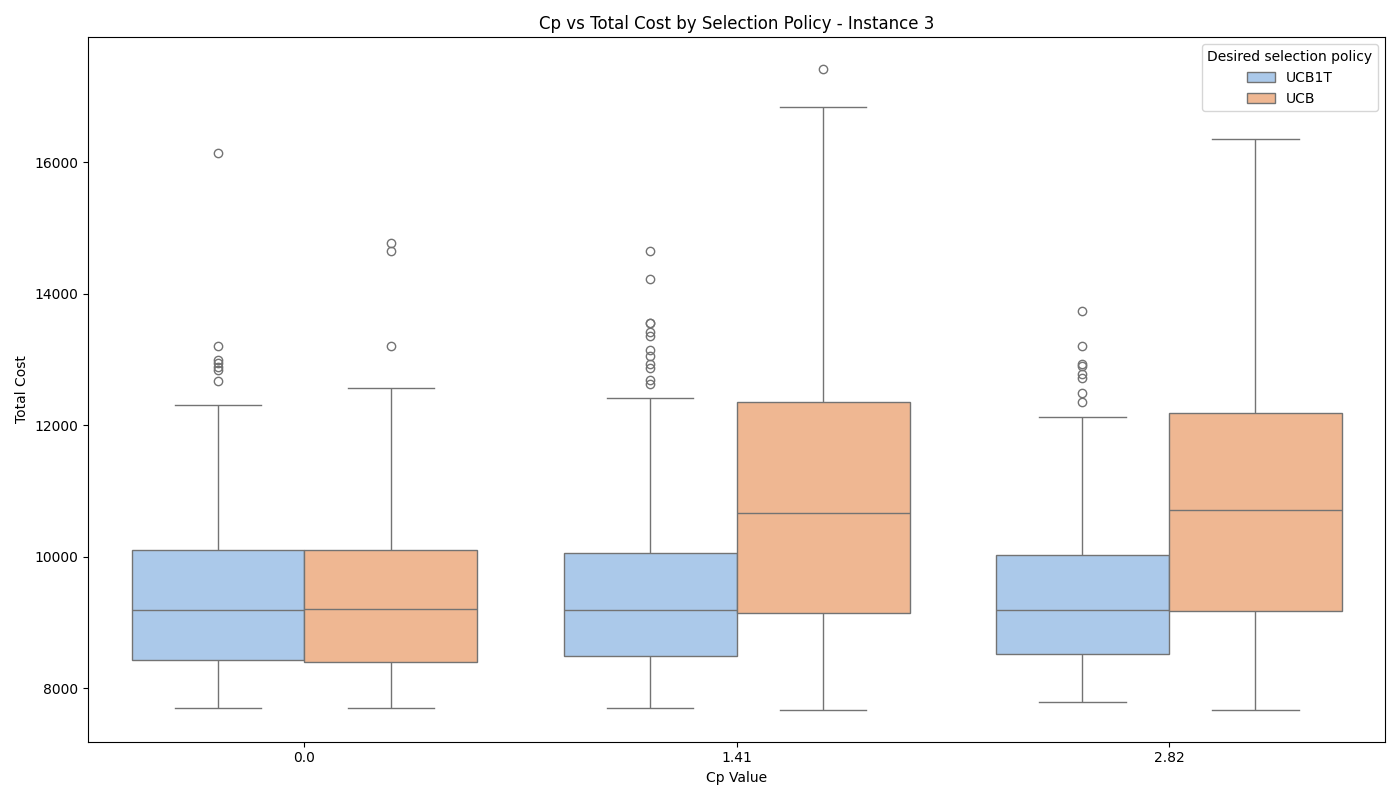
\includegraphics[width=\textwidth]{Figures/3 - cp_vs_cost.png}
    \caption{$C_p$ vs Total cost}
    \label{fig:cp_vs_cost_3}
\end{figure}
While UCB1T may require more time to converge, it generally explores the search tree more effectively, leading to better overall performance. One can notice that $C_p$'s correlation with the UCB1T selection policy for $I_3$ is low.



\newpage
\subsubsection*{Analysis of Expansion ratio}

\begin{figure}[!ht]
    \centering
    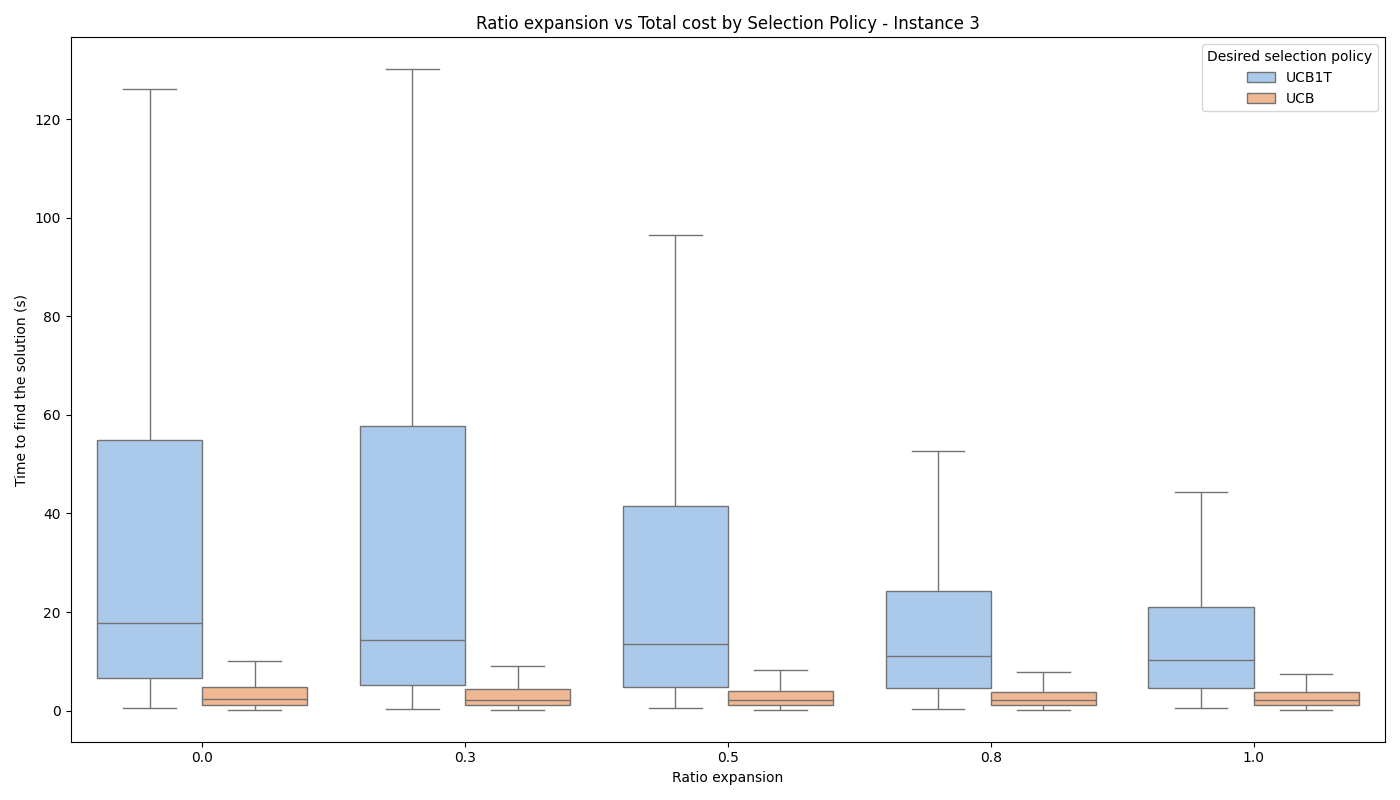
\includegraphics[width=\textwidth]{Figures/3 - ratio_vs_time.png}
    \caption{Ratio expansion vs Time to find the solution}
    \label{fig:Ratio vs Time}
\end{figure}

The box plots show the relationship between ratio expansion (the proportion of expanded child nodes that has the cheapest flight connection over the chosen number of children) and the time to find a solution for the UCB and UCB1T policies:

\begin{itemize}
    \item \textbf{UCB finds solution faster than UCB1T:}
          Across all ratio expansion values, the UCB policy consistently finds solutions more quickly than UCB1T. This suggests that UCB, being less aggressive in exploration, converges on solutions faster.

          %\item \textbf{UCB1T Takes Longer Due to Extensive Exploration:}
          %      UCB1T shows higher and more variable times to find solutions, especially at lower ratio expansions (e.g., $0.0$). This reflects UCB1T's property to explore more than UCB.

    \item \textbf{Higher ratios lead to a faster convergence:}
          For both policies, the time to find a solution generally decreases as the ratio expansion increases, indicating a more efficient search process when expanded nodes are less chosen randomly from the set of available actions. However, in more complex instances, it is crucial to have a ratio $r \in [0.3,0.7]$ to escape potential leaf node.
\end{itemize}

Finally, the UCB policy is more correlated to the expansion ratio than the UCB1T as shown in Figure \ref{fig:ratio_vs_cost_3}. UCB's overall performance is worst than UCB1T because it relies heavily on the exploitation compared to UCB1T that even if it converges slower gives better results.

\begin{figure}[!ht]
    \centering
    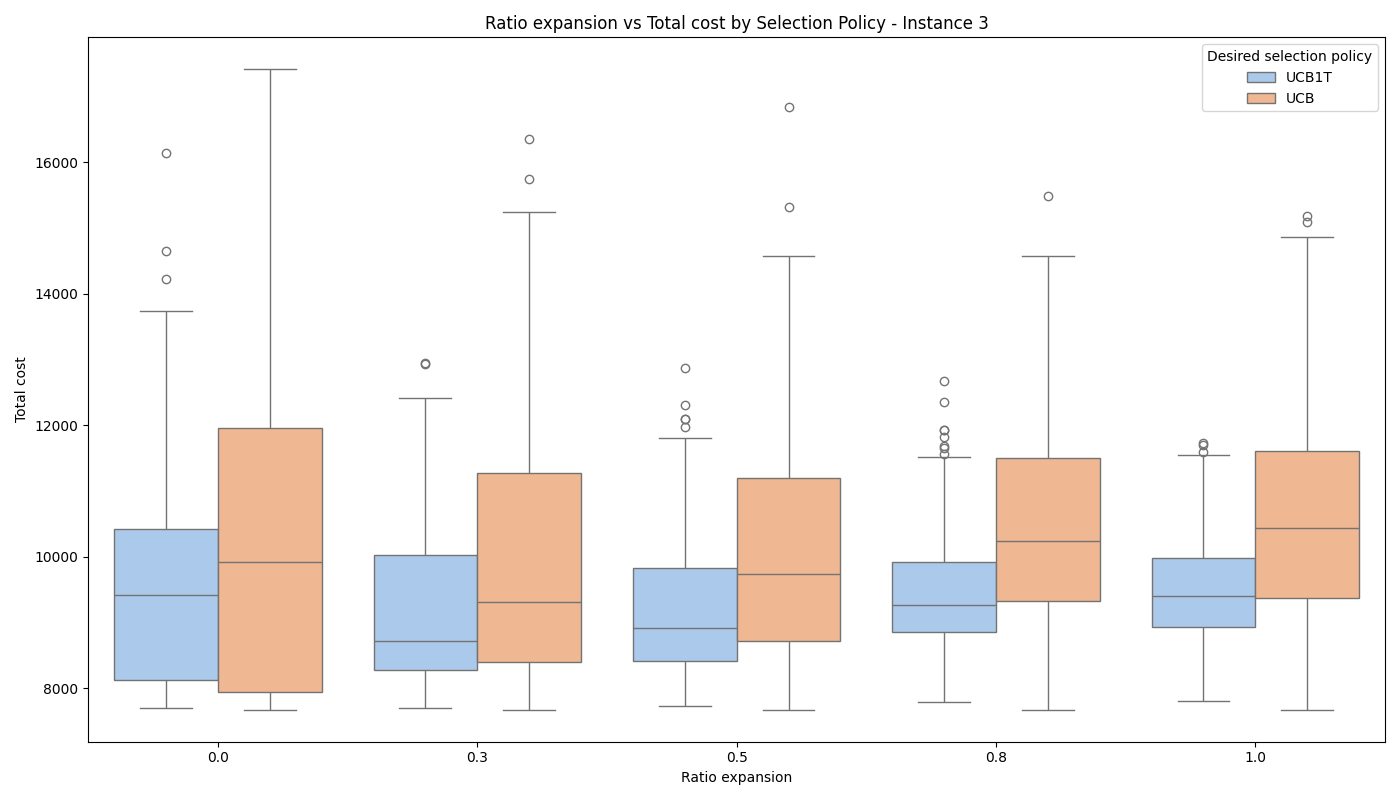
\includegraphics[width=\textwidth]{Figures/3 - ratio_vs_cost.png}
    \caption{Expansion ratio vs Total cost}
    \label{fig:ratio_vs_cost_3}
\end{figure}
\newpage
\newpage
\subsubsection*{Analysis of simulations performances}
\begin{figure}[!ht]
    \centering
    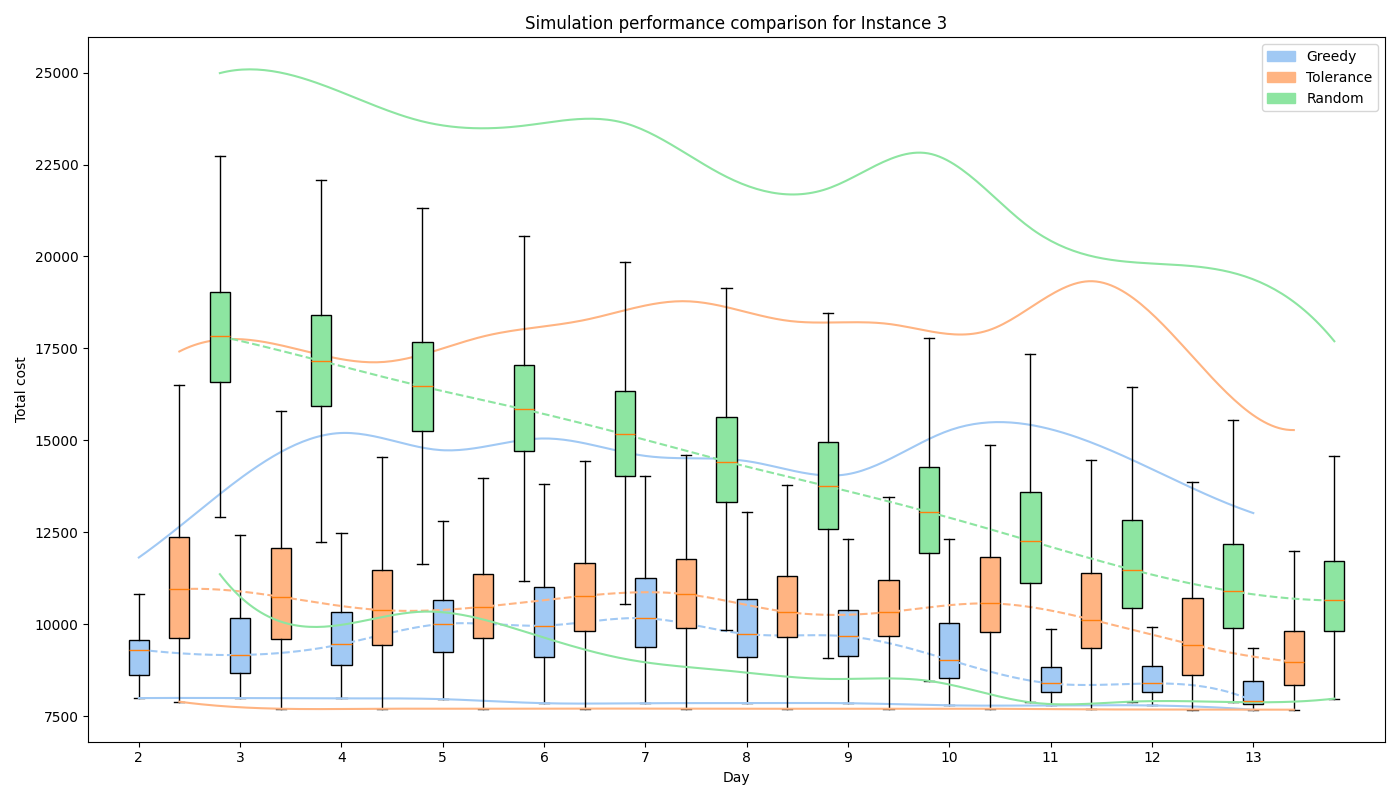
\includegraphics[width=\textwidth]{Figures/3 - Simulation performance.png}
    \caption{Simulation performance - Instance 3}
    \label{fig:sim_perf_3}
\end{figure}
Box plots for the tree simulations policies are represented on Figure \ref{fig:sim_perf_3}. For each day, the distribution of the simulated outcome is plotted regarding the simulation policy. Colored curves represent the minimum and maximum of these distributions, while dashed lines indicate the medians.

In Figure \ref{fig:sim_perf_3}, the greedy simulation policy is more performant because the distribution of simulations at every day has a lower min, max and median.
The convergence of the Random policy is more pronounced due to the policy's inherent randomness. For instance, with the greedy and tolerance policies, at day two or three, the minimum has already almost been reached. Therefore, a well-calibrated set of parameters for the $\mathcal{MCTS}$ (as defined in Section \ref{sub:notations}) should converge towards the minimum cost found during the simulations. If this is not the case, it indicates that the parameterisation of $\mathcal{MCTS}$ is not optimal. In Figure \ref{fig:sim_perf_4_cp_zero}, the distributions of the simulated outcomes are represented for a  $\mathcal{MCTS}(S_p(C_p=0),E_p(c),R_p,N_c=10)$.


\begin{figure}[!ht]
    \centering
    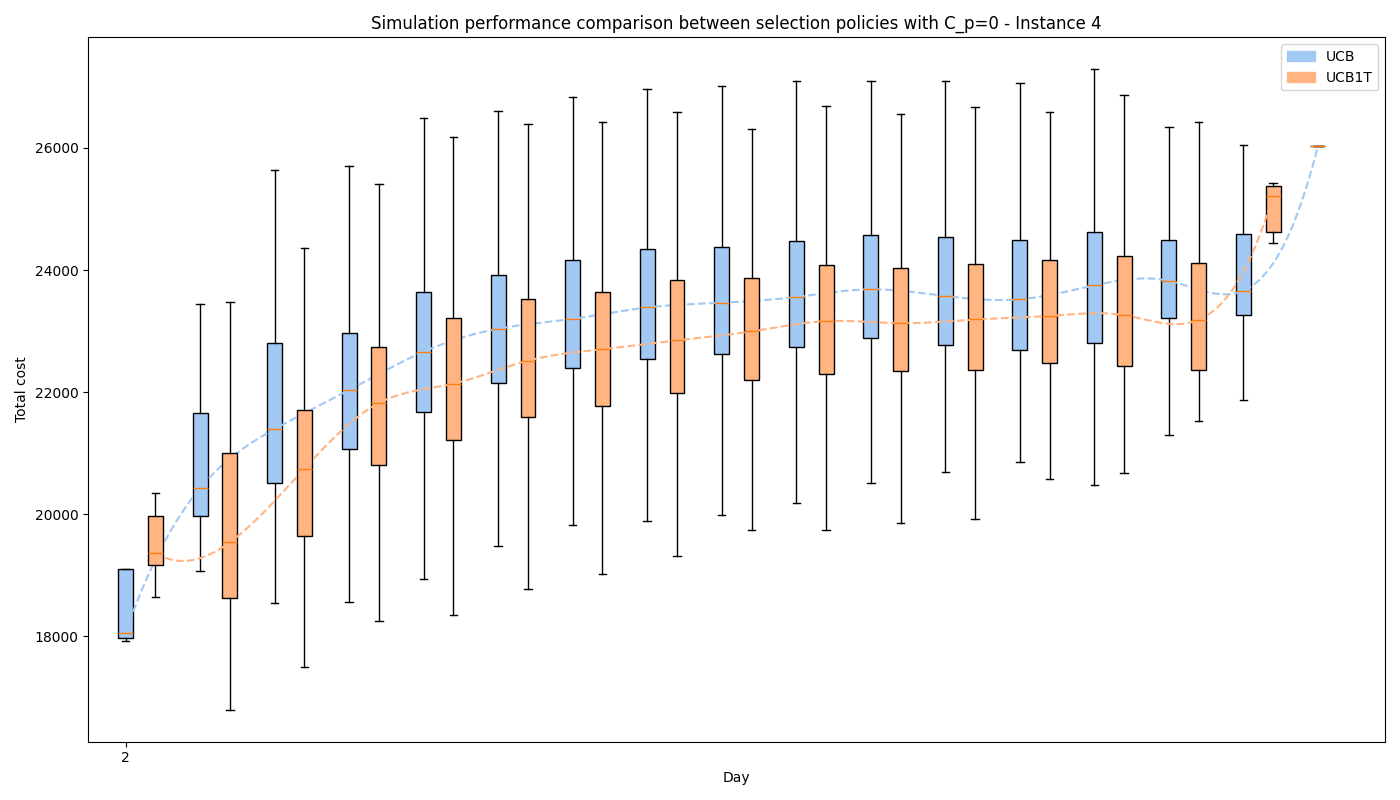
\includegraphics[width=\textwidth]{Figures/4 - Simulation performance - CP=0.png}
    \caption{Simulation performance $C_p=0$ - Instance 4}
    \label{fig:sim_perf_4_cp_zero}
\end{figure}
The parametrisation of this MCTS is not efficient for the considered instance, hence the search process do not converge towards the minimum found cost. These two distributions have a similar behavior, having $C_p=0$ indicates a similar decision-making process when using the UCB and UCB1T selection policy.

In Figure \ref{fig:sim_perf_vs_c_3}, the median distributions for the different scenarios have been plotted. One can observe that having a value $c$ too close to 1, does not on average converge to this minimum-cost solution. A contrario, lower $c$ values appears to guide the tree search more effectively during the first days of simulations, which is crucial to not overexpand the size of the tree, which can lead to an inefficient and time-consuming MCTS.
\begin{figure}[!ht]
    \centering
    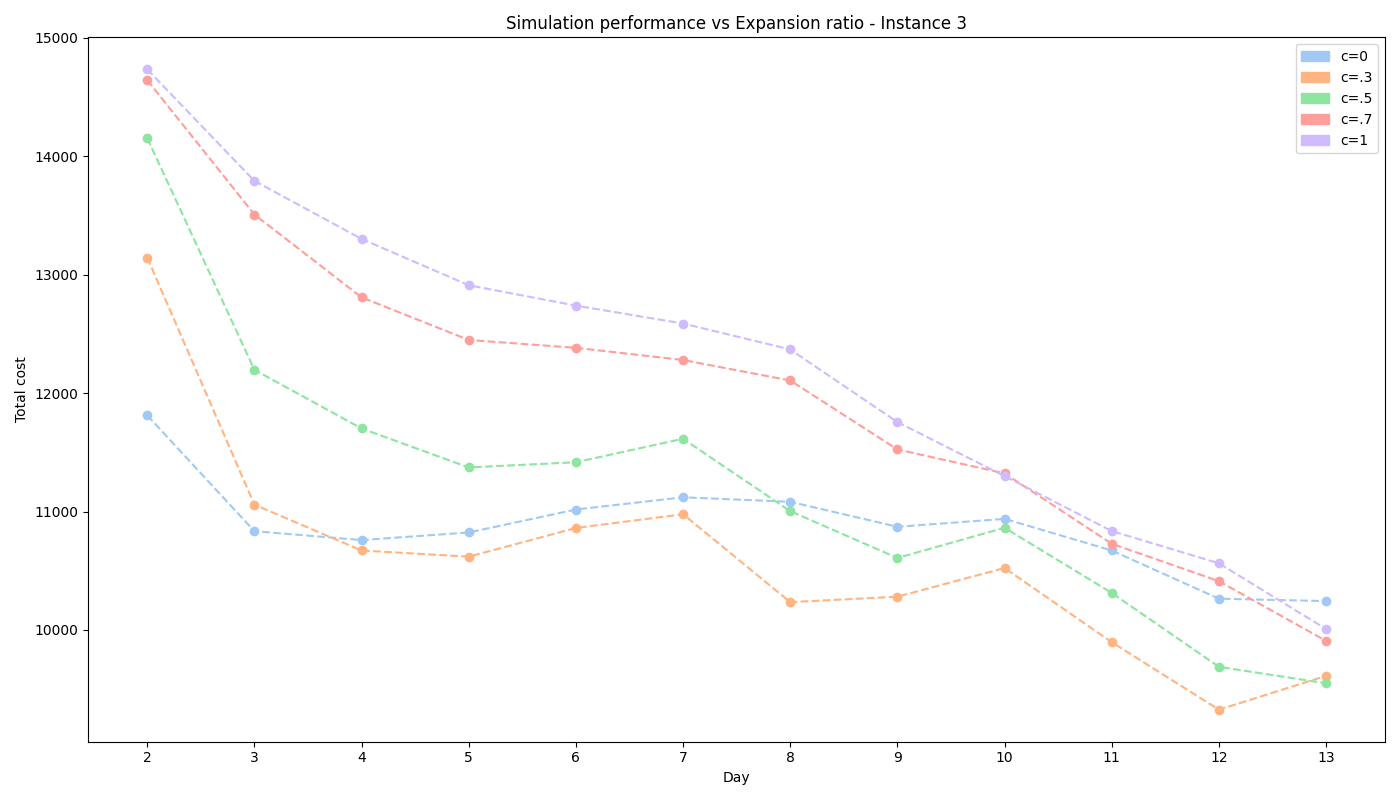
\includegraphics[width=\textwidth]{Figures/3 - Simulation performance vs Expansion ratio.png}
    \caption{Simulation performance vs Expansion Ratio - Instance 3}
    \label{fig:sim_perf_vs_c_3}
\end{figure}

These conclusions can be drawn for small instances, however for $I_4$, we can clearly see in Figure \ref{fig:sim_perf_vs_c_4} that having $c=0$ for a greedy selection policy is inefficient in this tree search because it diverges from the min-simulated cost. The tree search is therefore unable to find a solution after 10 minutes. Based on the median comparison, $c=1$ is a more optimal parameter for guiding the tree search (for $I_3$).
\begin{figure}[!ht]
    \centering
    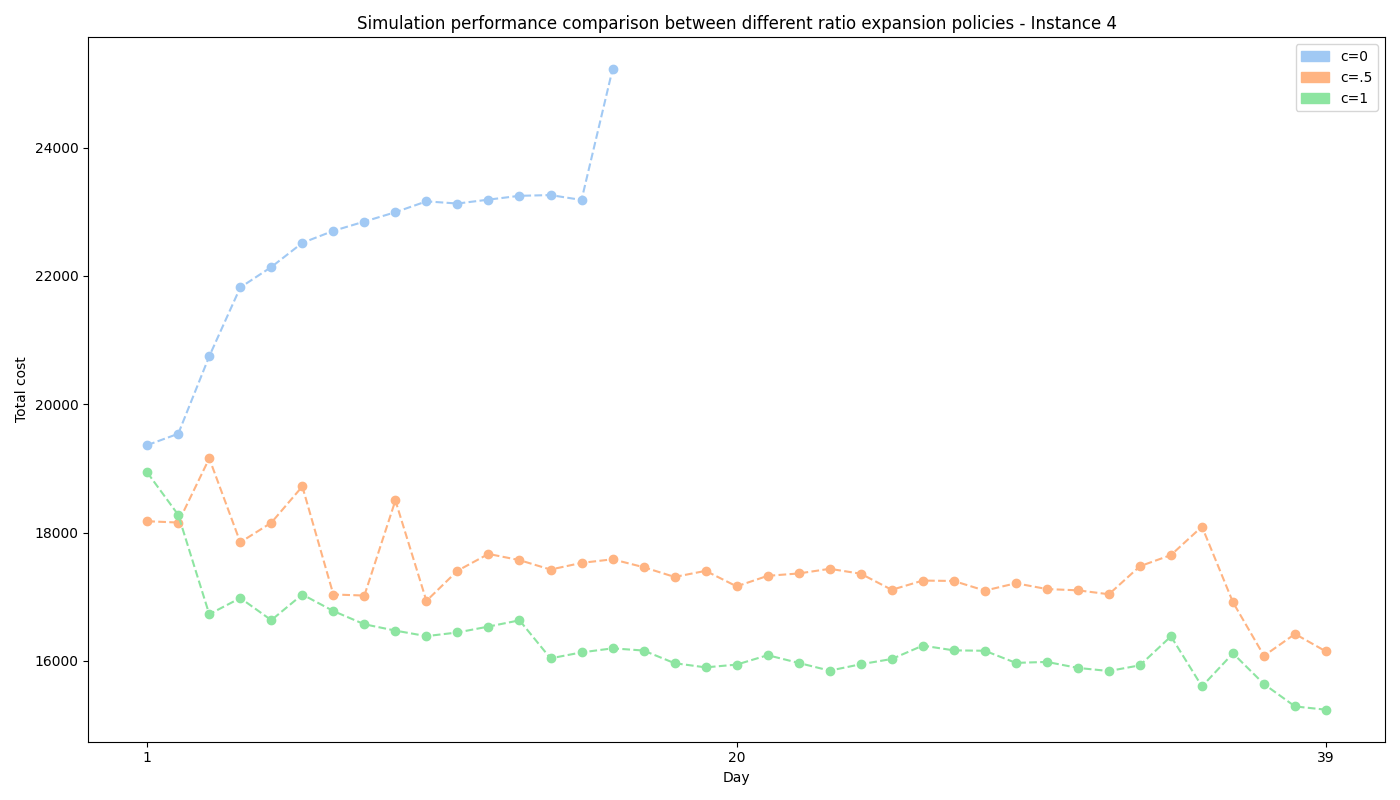
\includegraphics[width=\textwidth]{Figures/4 - Simulation performance vs Expansion ratio.png}
    \caption{Simulation performance vs Expansion Ratio - Instance 4}
    \label{fig:sim_perf_vs_c_4}
\end{figure}

\subsubsection*{Correlation}
\begin{figure}[!ht]
    \centering
    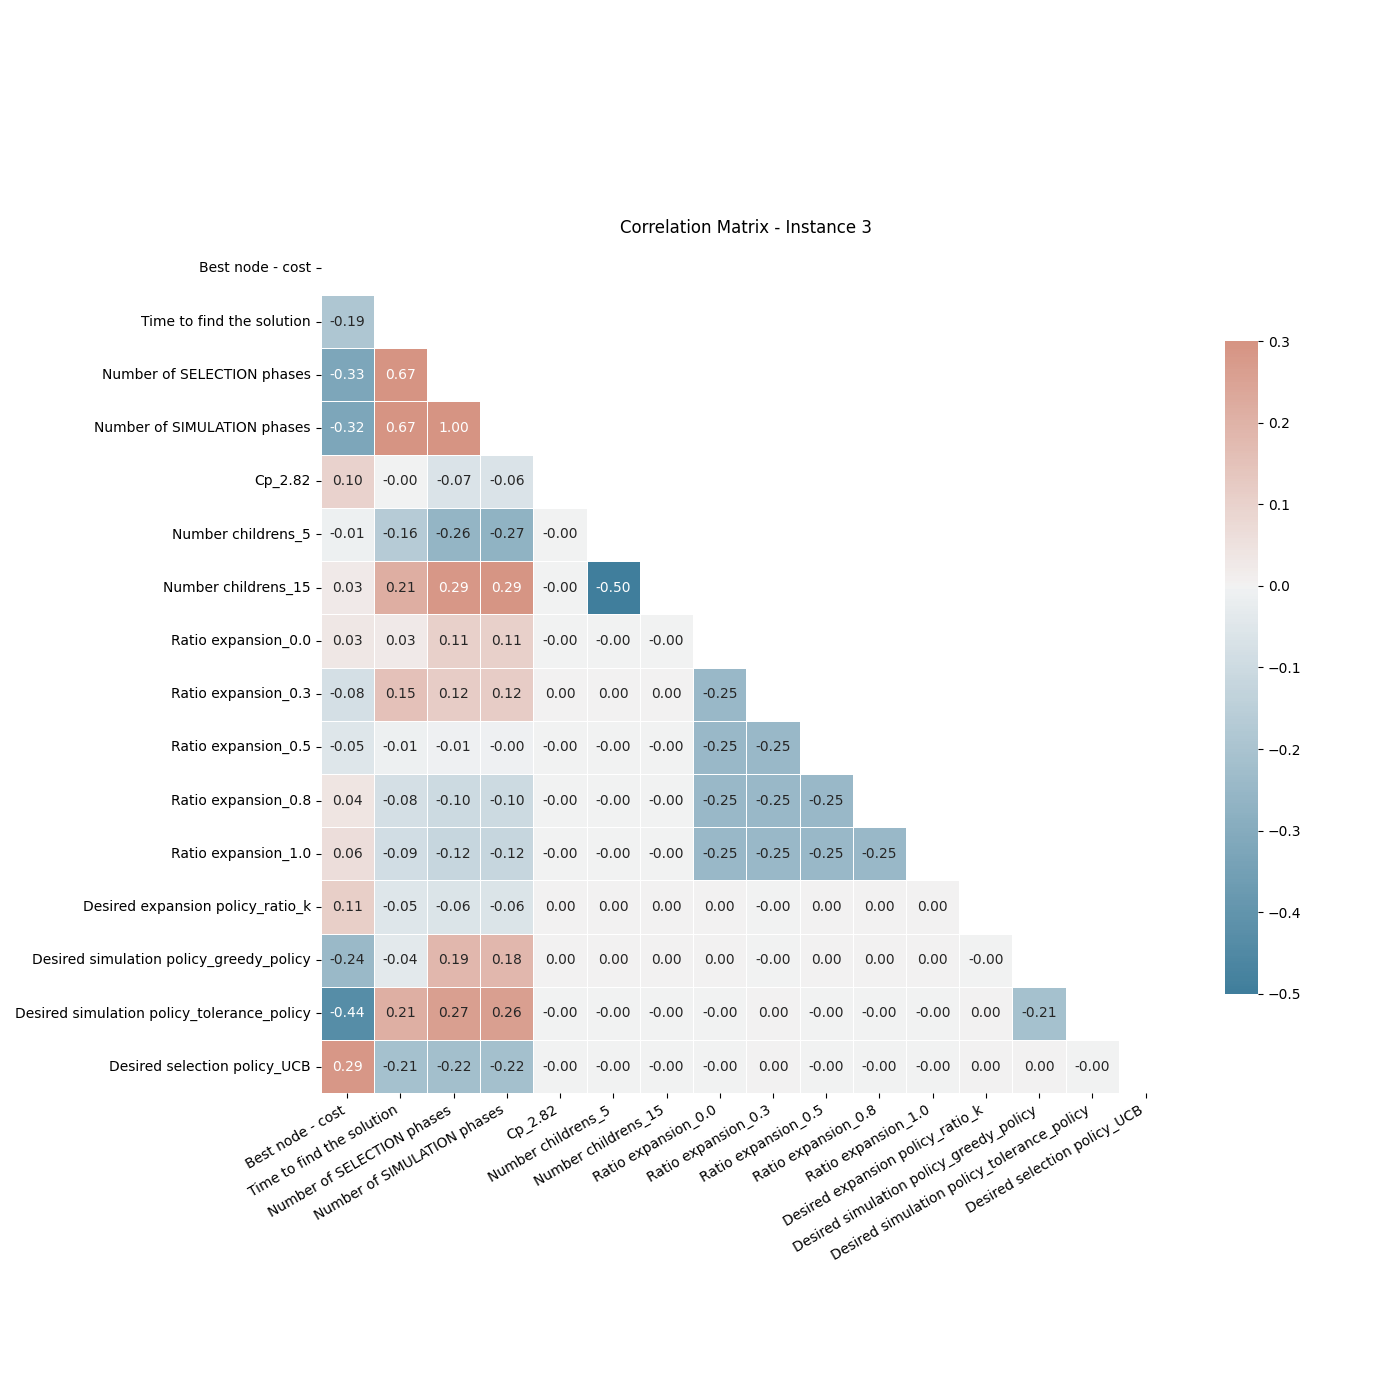
\includegraphics[width=\textwidth]{Figures/3 - correlation_matrix.png}
    \caption{Correlation matrix - Instance 3}
    \label{fig:corr_3}
\end{figure}
\newpage
\newpage
\subsection{Parallelisation}
As discussed in Section \ref{sub:parralelisation}, parallelisation can be implemented to better estimate one selected node's value.
In our implementation, for $I_4$, we parallelisation a $\mathcal{MCTS}(S_p(C_p=0)="UCB",E_p(c=0)="ratio\_k",R_p="random",N_c=10)$ on five cores. The set of parameters has been chosen to represent the behavior of parallelisation in a stochastic environment.  The parralelisation has been implemented during the simulation process. Therefore, we chose the minimum outcome of the five simulations.

In Figure \ref{fig:sim_perf_parral_4}, the five cores parallelised's distribution better performs than the non-parralelised approach. It confirms that parallelisation guides the MCTS more effectively in the first days of the tree search.

\begin{figure}[!ht]
    \centering
    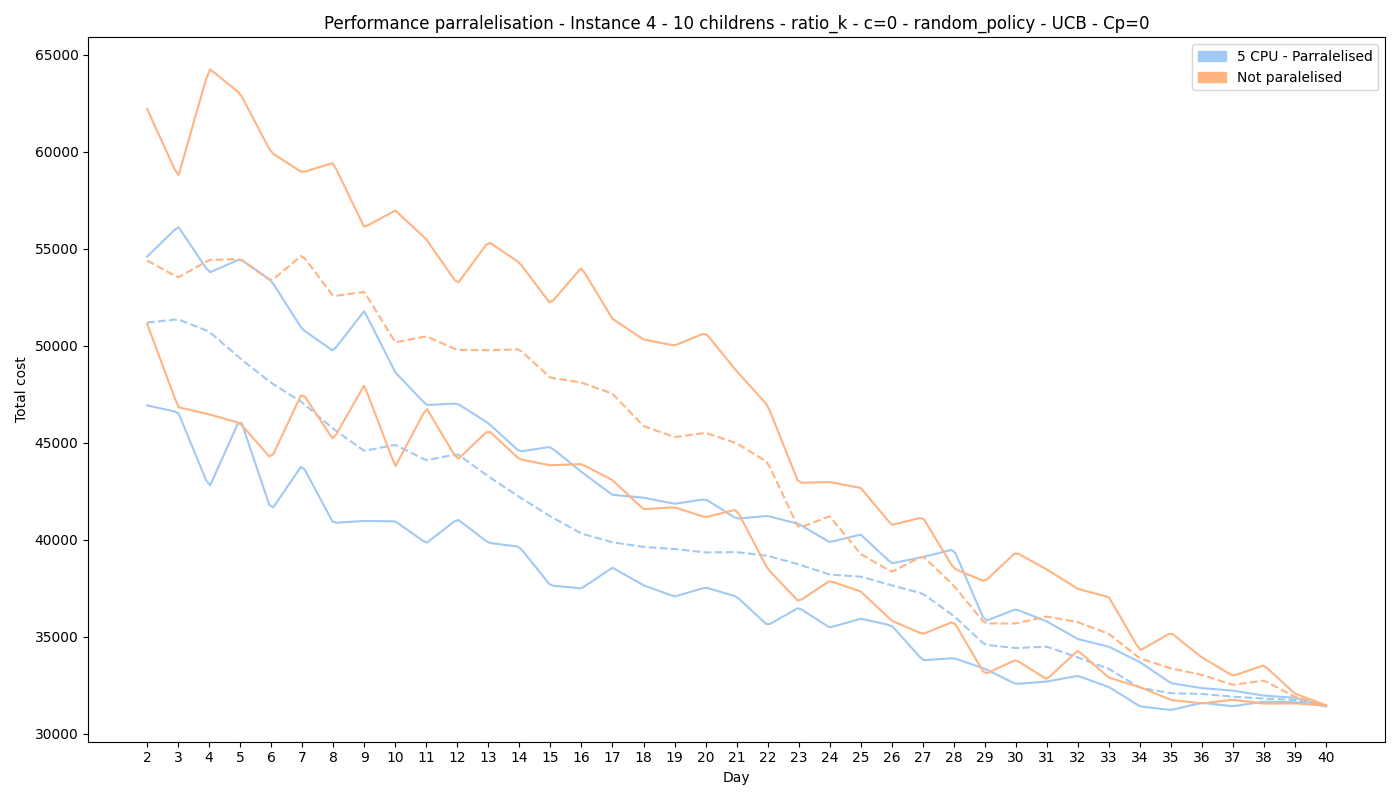
\includegraphics[width=\textwidth]{Figures/4 - Paralelised vs 5 CPU paralelised.png}
    \caption{Performance Parrelisation vs no - Instance 4}
    \label{fig:sim_perf_parral_4}
\end{figure}

\begin{figure}[!ht]
    \centering
    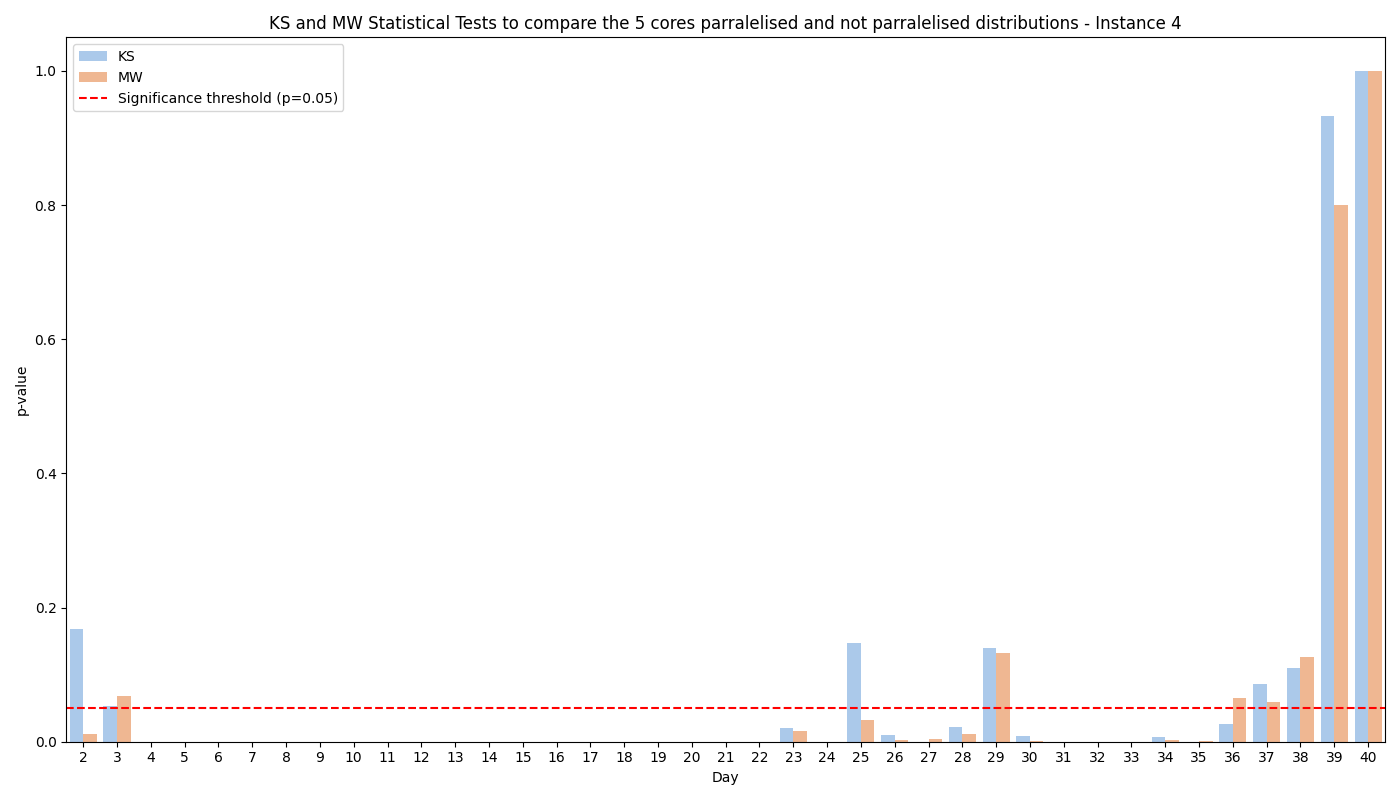
\includegraphics[width=\textwidth]{Figures/Distribution stats tests P vs NP.png}
    \caption{Stats test Performance Parrelisation vs no - Instance 4}
    \label{fig:stats test parralel}
\end{figure}
The Mann-Whitney and the Kolmogorov-Smirnov statistical tests have been implemented. These tests compute p-values that test the null hypothesis that the two groups have the same distribution. Hence, from Figure \ref{fig:stats test parralel} there is enough statistical evidence to say that a five core parallelised MCTS with a stochastic simulation policy better performs with parralelisation at a 5\% level.

A comparison between five-core and ten-core parallelisations of the considered Monte Carlo Tree Search (MCTS) is shown in Figure \ref{fig:parralel (5 vs 10)} and \ref{fig:Stats test 5 VS 10 Parall}. There are no statistical improvments in increasing the number of cores. As discussed in \cite{different_selection_policies}, too many modifications to the MCTS can lead to undesirable behaviour.

\begin{figure}[!ht]
    \centering
    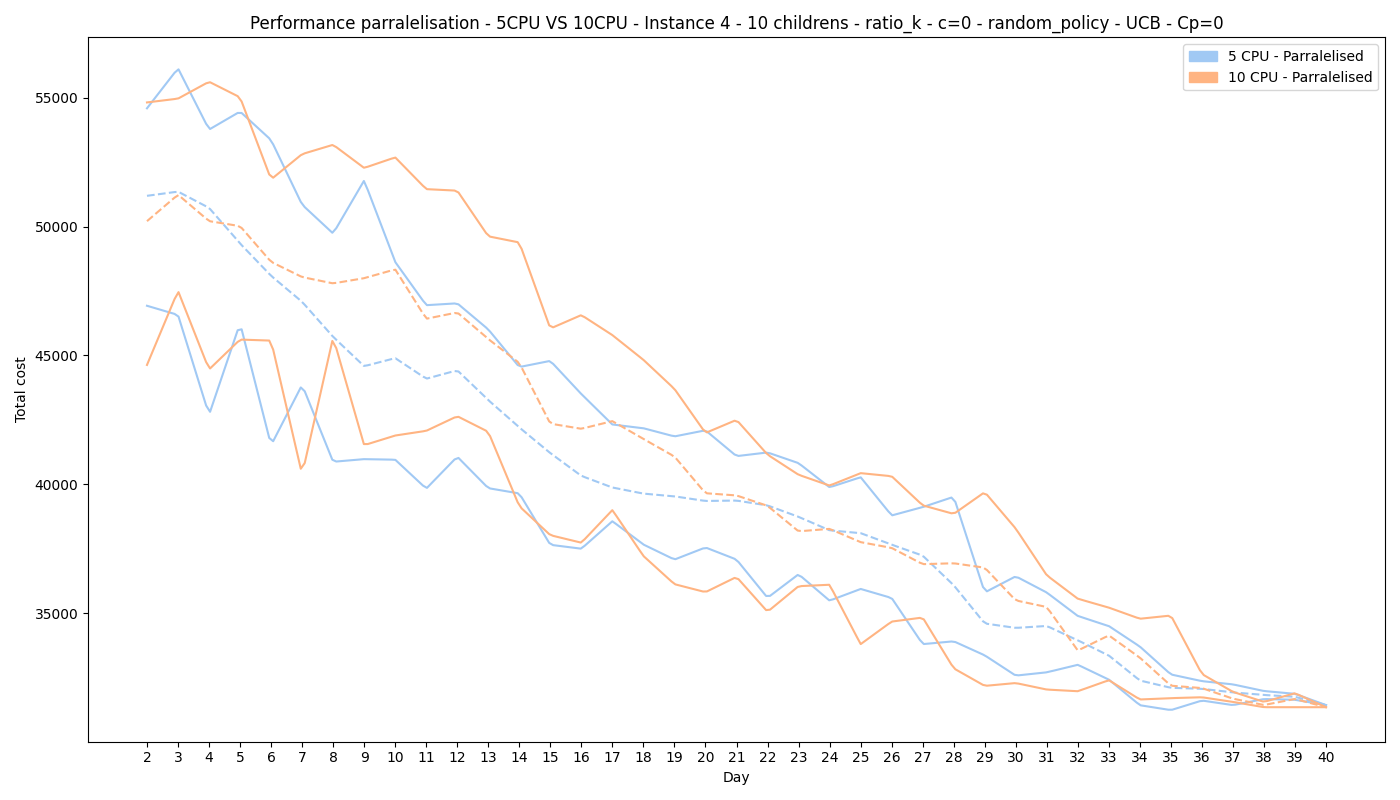
\includegraphics[width=\textwidth]{Figures/4 - 5 CPU Paralelised vs 10 CPU paralelised.png}
    \caption{test Performance 5 and 10 Parrelisation vs no - Instance 4}
    \label{fig:parralel (5 vs 10)}
\end{figure}


\begin{figure}[!ht]
    \centering
    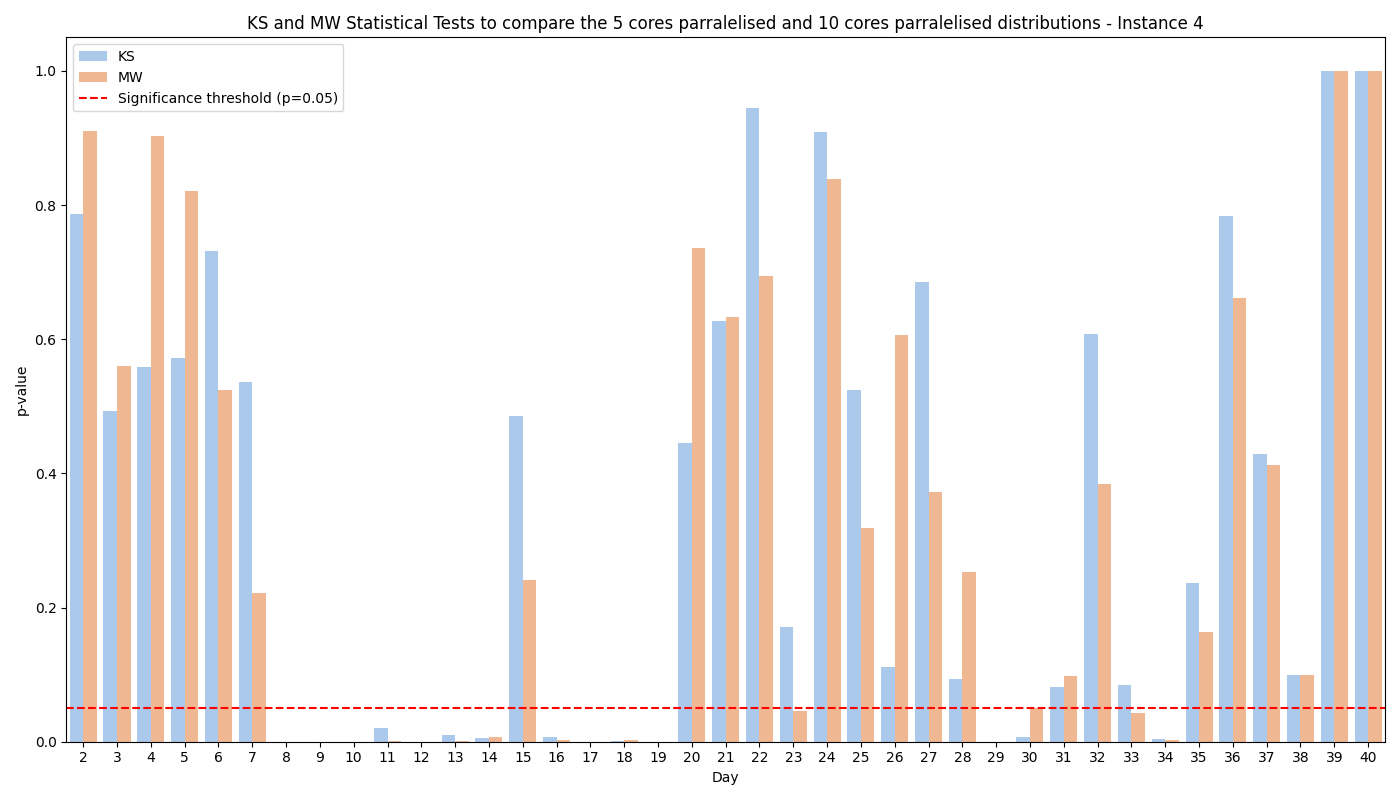
\includegraphics[width=\textwidth]{Figures/4 - Distribution stats tests 5P vs 10P.png}
    \caption{Stats test Performance 5 and 10 Parrelisation vs no - Instance 4}
    \label{fig:Stats test 5 VS 10 Parall}
\end{figure}

\newpage
\subsubsection{$I_5$ and $I_6$}

The challenge faced with these two instances is that with the defined grid search, the $\mathcal{MCTS}$ function was not able to conduct the tree search effectively.

Chosen nodes for the simulation that reached final states, under random or tolerance policies, failed to progress further the expansion of the tree because of the randomness of these simulations. Hence, as decided during the implementation of the algorithm, if a simulation from a node cannot reach a final state, this node would be deleted.
\subsubsection{$I7$ and $I_8$}

